\chapter{Implementation Use Case:  Restaurant Recommendation }
\label{chap:restaurant}
\section{Overview}

In this chapter, we demonstrate how Socrates Sim was adapted to support the restaurant domain. We start with a dialog agent that makes restaurant recommendations. The objective of Socrates Sim will be to produce a set of simulated conversations between a user simulator and the dialog agent. The user simulator will emulate a human user and come into the conversation with a hidden goal (for example, get the name and phone number for a Greek restaurant). The dialog agent will attempt to elicit as much information about the user's preferences and then attempt to provide a useful recommendation.  In this task completion exercise, either the user or the dialog agent can take the first turn. 

As mentioned in the previous chapter, the framework requires knowledge of the dialog domain, the path locations of the user simulator and dialog agent, and the simulation settings. We will walk through how each of those components are created and then used to run simulations on Socrates Sim.

\section{Defining the Dialog Domain}

We use the Dialog State Tracking Challenge 2 (DSTC2) restaurant recommendation ontology and data for our use case. The DSTC2 was a research challenge put together by the University of Oxford and Microsoft to advance dialog research. For DSTC2, the goal was to track the state of multi-stage conversations between real humans and an expert restaurant recommender service. The recommender service provides recommendations based on the following user preferences: cuisine, area, and price range. DSTC2 provides a rich and deep set of training data that was used to train models for the natural language generation (NLG) and the natural language understanding (NLU) components of the use simulator.

The first thing we do is create the dialog domain configuration file (see Figure \ref{fig:restaurant_domain}). This file is used to generate a domain object that will be used by the dialog manager, user simulator, and dialog agent. We use the dialog DSTC2 ontology to define the dialog acts, slots and slot values in the domain configuration file. To simplify the use case, we did narrow down the dialog act options. The request and inform slots and slot values are the same. 

\begin{figure}[h!]
	\centering
	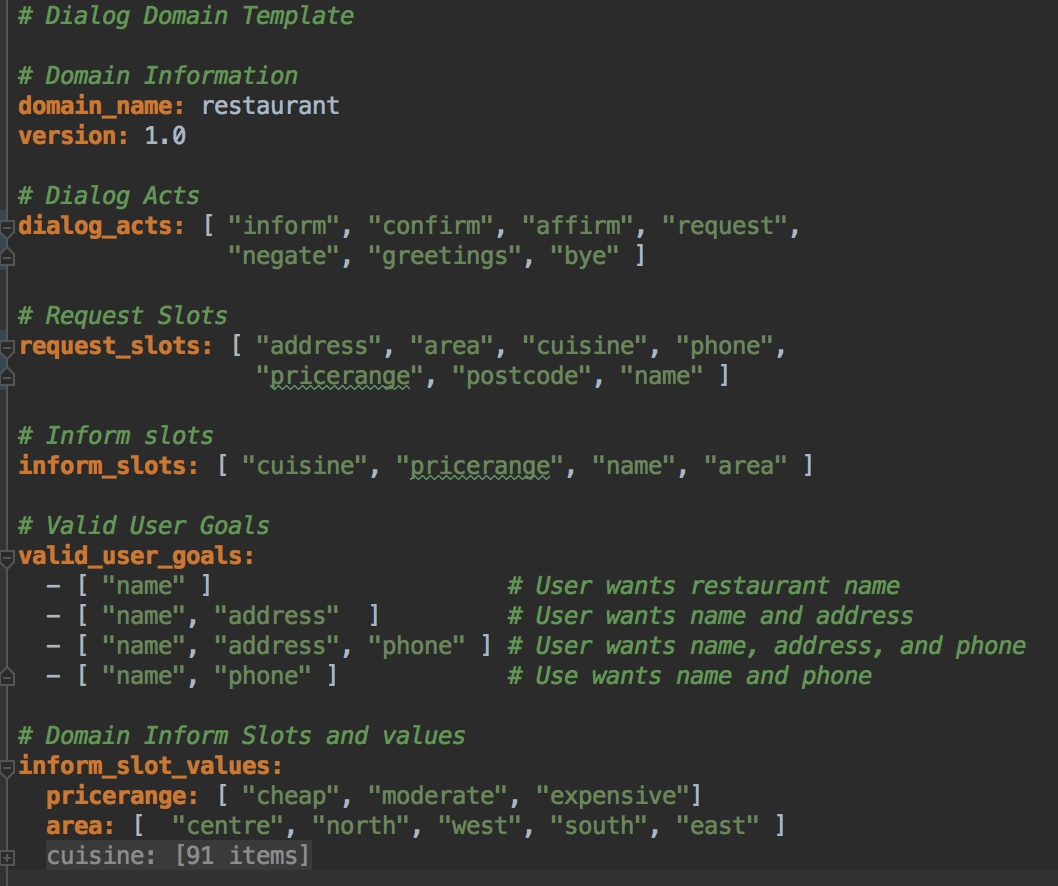
\includegraphics[scale=.25]{diagrams/sample_domain.jpeg}
	\caption{ Restaurant dialog domain configuration file. }
	\label{fig:restaurant_domain}
\end{figure}

One important and novel feature of this file is the valid user goal templates section. It specifies the valid goals a user is allowed to have when engaging the dialog agent. That section enumerates the various combinations of required request slots that must be present in the user goal.

The knowledge base for this use case is a csv file with the various restaurants from the Cambridge (UK) area. Each row represents a unique restaurant and the column values capture the restaurant's cuisine, price range, area, phone number, and address. The data was scraped from Yelp.com. The restaurants' list is loaded into memory as a \textit{DomainKBtable} object. The knowledge base is converted into a pandas dataframe and the class provides a set of methods for querying. The knowledge base is primarily used by the dialog agent to make recommendations.

\section{User Simulator Implementation}

In this section, we describe the implementation of a rule-based user simulator. The user simulator is initialized with a set of hidden preferences (see Figure \ref{fig:ex_user_goal}) and aims to get the name of a restaurant that satisfies those preferences from the dialog agent. Additionally, the user simulator may also want the restaurant's phone number and address.

\begin{figure}[h!]
	\label{fig:ex_user_goal}
	\begin{lstlisting}
	inform_slots:
		cuisine: "chinese"
		pricerange: "cheap"
	request_slots:
		name: "UNK"
		phone: "UNK"		
	\end{lstlisting}
	\caption{ Example user goal. User is seeking the name and phone number of a cheap Chinese restaurant}
	
\end{figure}

\pagebreak

In order to integrate the user simulator into Socrates Sim, we define an interface class that is the descendant of the \textit{Speaker} abstract base class. Our rules-simulator class is implemented as a subclass of the \textit{UserSimulator} class. The rules-simulator needs to implement four key public methods: \textit{reset}, \textit{next}, \textit{get\_utterance}, and \textit{parse\_utterance}. 

At the start of each simulation round, the dialog manager calls the user simulator's \textit{reset} method. The purpose of the \textit{reset} method is to set a user goal and reset the user simulator's internal state. The dialog manager passes a new \textit{DialogGoal} object to the \textit{reset} method. In this method, we also reset the enum value of \textit{DialogStatus} to NOT\_STARTED and current turn to -1.

The primary logic of the user simulator is captured in the \textit{next} method, which we describe in \ref{sssec:logic}. The nlg and nlu processes are implemented as separate classes and described further in detail below. To demonstrate the versatility of the simulator, we implement both a rule-based and model-based approach for both the nlu and nlg. We can easily swap out implementations in the simulation configuration file, without having to modify the user simulator code directly.

\subsection{Simulator Logic}
\label{sssec:logic}

The internal logic for the user simulator is driven by the user agenda. The user agenda captures what the user simulator will communicate to the dialog agent. For our implementation, we simply concatenate the inform and request slots stored in the user goal. 

\cite{Schatzmann2009TheHA} formally define the user agenda as a stack-like structure containing the pending dialog acts that user will say over the course of the conversation. All key-value pairs captured in the corresponding inform and request slot lists are mapped to inform and request dialog acts. Over the course of the dialog, the top item on the stack, which gets popped, contains the dialog action for what the user simulator will do next. That action is passed to the simulator's internal nlg process to generate a new speech utterance. 

For memory efficiency, we do not actually implement the agenda as an explicit stack. The information already exists in the user goal. Instead, we pop directly from the inform slots list in the user goal in response to the dialog acts from the dialog agent. We keep track of the conversation state by checking how many of the request slots have been filled with real values. The rules-simulator runs sequentially through the request slots at the end of each conversation and updates its internal\textit{ DialogStatus} enum object with one of two values: NO\_OUTCOME\_YET or FINISHED.

The logic for how the user simulator responds to incoming speech acts from the dialog agent is handled by the \textit{next} method. 

\begin{figure}[h!]
	\label{fig:dispatch_tree}
	\begin{lstlisting}
	response_router = { 
		"greetings": respond_general,
		"inform": respond_to_suggestion,
		"random_inform": respond_random_inform,
		"request": respond_request,
		"confirm": respond_confirm,
		"bye": respond_general
	}	
	\end{lstlisting}
	\caption{ Internal dispatch tree for the rules-simulator. }
\end{figure}

The user simulator first parses the agent's incoming dialog action and then responds to it using an internal dispatch tree (see Figure \ref{fig:dispatch_tree}). The dispatch tree is implemented as a Python dictionary, where the dialog acts are mapped to resolver functions. Each response function has the same method signature.  The response functions take in a \textit{DialogAction} object and return a new \textit{DialogAction} object that represents the user's response to the dialog agent. 
 
How the resolvers handle the greetings, bye, and confirm responses is straightforward. The resolver simply invokes the \textit{NLG} object's \textit{get\_utterance} method and sends a response dialog action. In the greetings case, if the rules-simulator is the first speaker, it will randomly pop a subset of its inform slots that will be used to inform the dialog agent. 

The resolver for responding to the agent's request actions is a bit more complicated. The simulator will look at the parsed request slots types the agent is asking about and attempt to find the corresponding inform slots in its \textit{DialogGoal} object. For example, if the dialog agent asks \textit{What cuisine do you prefer?}, the simulator will look up cuisine in its internal goal object and return the answer Chinese (based on the goal in \ref{fig:ex_user_goal}). For the case where the requested slot type is not found in the user's inform preferences, the simulator will respond with either\textit{ I don't know} or \textit{I don't care}. This null response can be configured in the simulation configuration file, where the response is either set to one of those two options or randomly chosen. Additionally, to simulate a realistic user, at configuration time, the researcher can also set the probability with which the simulator will \textit{lie} or \textit{change its mind } about its preferences. In those cases, the simulator will randomly sample the provided slot values in the dialog domain object and return a different slot value. If rules-simulator has informed the dialog agent of all its preferences, the simulator will then pop values from its request slots and ask for a recommendation. 

The dialog agent will use the inform dialog act in order to provide the user simulator with new information (e.g., a restaurant suggestion or the restaurant's phone number). If the dialog agent sends an inform action, it will be routed to the inform resolver. This method updates the user simulator's request slots with newly provided information. So for example, if the dialog agent made the suggestion, \textit{Check out Golden Dynasty}, the \textit{UNK} value in \ref{fig:ex_user_goal} would be replaced by "Golden Dynasty". If all the \textit{UNK} values in the request slots are filled with real values, the user simulator will update its internal status to FINISHED and issue the bye action. 

\subsection{Natural Language Understanding}
The goal of nlu is to parse a natural language utterance and generate a semantic frame representation for the \textit{DialogAction} object. The parsed dialog action contains the intent of the utterance, i.e. the dialog act, and any entity/entity types, i.e. the dialog parameters, which are contained in the utterance. We implement two different nlu strategies to demonstrate the versatility and modularity of Socrates Sim. The first approach leverages a combination of simple NLP rules and some basic heuristics. We call this approach the rule-based approach. The second approach is model-based, where we trained a neural machine translation model to translate a natural language utterance into a semantic frame representation. 

Since the nlu process is abstracted from the user simulator, we created an interface class to invoke the nlu logic for both approaches. We created the \textit{NLUSimple} and \textit{NLUModel} classes to support each approach accordingly. Both classes are implementations of the\textit{ NLU} abstract base class. 

\subsubsection{rule-based NLU}
~ \\
For the rule-based approach, our parser has a two-part strategy. The first is to classify the intent of the utterance and map it to a dialog act. The second is to run an entity extraction pass and attempt to extract the entities contained in the utterance and map them to inform slot types.

The algorithm for the intent classification consists of two parts. The first is running the utterance through a question classifier (implemented from \cite{chewning_lord_yarvis_2015}). If the utterance is a question, we classify it as a request dialog act. Otherwise,we run the utterance through a set of regular expression matches and return the corresponding dialog acts (see \ref{fig:intent_clf}). Given the wide range of potential string matches for inform, we use \textit{inform} as the default dialog act. 

\begin{figure}[h!] 
	\label{fig:intent_clf}
	\begin{lstlisting}
	Classify Intent
	input: natural language utterance
	
	IF input is a question:
		return 'request'
	ELSE IF input contains [you, you want, right?]:
		return 'confirm'
	ELSE IF input contains [yes, yeah, yup, correct, right]]:
		return 'affirm'
	ELSE IF input contains [no, nope, wrong, incorrect]:
		return 'negate'
	ELSE IF input contains [hi, hello]:
		return 'greetings'
	ELSE IF input contains [bye, goodbye, thanks, thank you]:
		return 'bye'
	ELSE
		return "inform"
	\end{lstlisting}
	\caption{ Intent classifier algorithm}
\end{figure}

After the intent is classified, we check to see if any entities are found in the utterance that can be mapped to known entity types. To achieve this, we first look up all the slot values defined in the domain object. Next, we create a reverse map dictionary, where each unique slot value (the entity) is mapped to a slot type (e.g., cuisine or price range). The nlu parser tokenizes the utterance into a set of word trigrams and checks if a slot type exists for the token in the reverse map. All positive matches are added to the dialog params list in the \textit{DialogAction} object. Finally, the parse utterance will return a \textit{DialogAction} object with parsed dialog act and a list of dialog parameters. 

\subsubsection{Model-based NLU}
~ \\
We also implement two simple neural machine translation models for our NLU module. The DSTC2 provides a large corpus of conversations between human users and a human expert posing as the dialog agent. Between the training and development sets, there are about 2,000 annotated calls. All speech utterances (between the human and agent) are annotated to include dialog act, inform/request slots and values.

Our first neural machine translation model is adapted from \cite{brownlee_2017}. It is a simple LSTM encoder-decoder model. We use Adam for optimization and categorical cross-entropy for the loss function. The model was implemented in Keras and trained over 100,000 epochs on 1,600 input calls. Unfortunately, the model performance was rather poor. It has a .6 cross-validation accuracy and a .45 accuracy against the test set. While this model is unusable, we do use it in the runtime performance evaluation, as it was simpler to incorporate the model into the simulation workflow. 

\begin{figure}[h!]
	\centering
	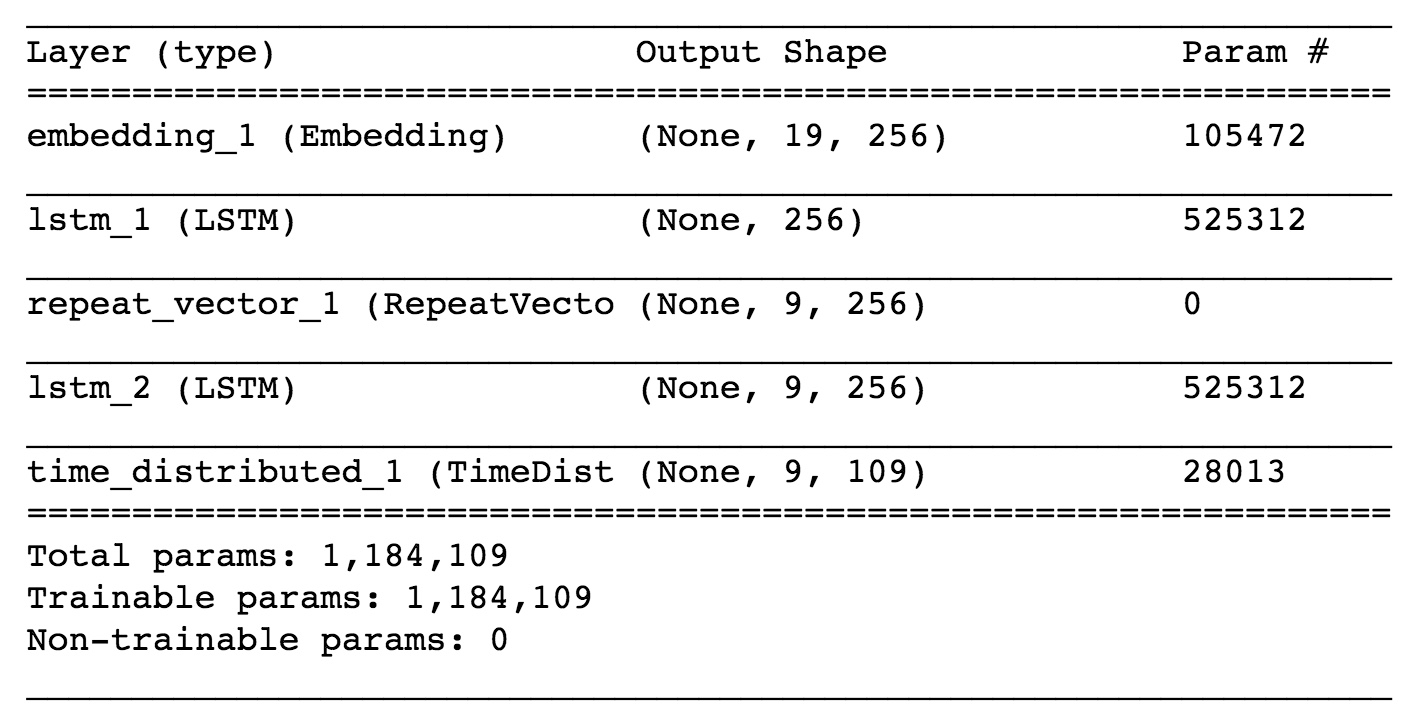
\includegraphics[scale=.25]{diagrams/simple_nmt.jpeg}
	\caption{ Neural machine translation model architecture  - \cite{brownlee_2017} }
	\label{fig:simple_nmt_model}
\end{figure}

Given the poor performance of the \cite{brownlee_2017} model, we trained a new neural-machine translation model using OpenNMT (\cite{2017opennmt}). OpenNMT is an open source neural-machine translation tool produced and maintained by Alexander Rush and the Harvard NLP group. We trained the model on 1,600 input calls and saw significant model performance improvement (cross-validation accuracy of .7 and test accuracy of .65). One of the limitations of this approach using OpenNMT is that the tool requires you to use its command line tool for generating new predictions. The library currently does not support programmatic access to the trained model. As a result, we had to develop a rather convoluted process to incorporate it into the Socrates Sim. Our \textit{NLUModel} class first writes the utterance to a text file. Next it invokes OpenNMT tool as a subprocess with the input text file. OpenNMT generates a prediction and writes it to an output text file. That file is read in and converted into a \textit{DialogAction} object. 

\begin{figure}[h!]
	\centering
	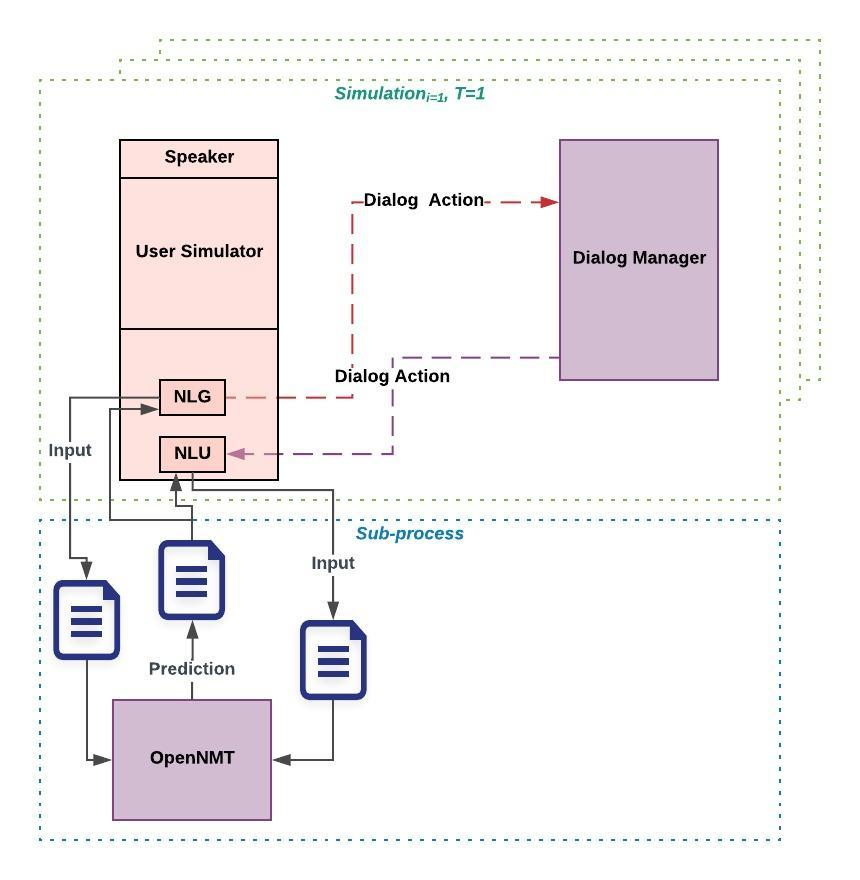
\includegraphics[scale=.65]{diagrams/open_nmt.jpeg}
	\caption{ NLU process using OpenNMT. }
	\label{fig:open_nmt_model}
\end{figure}


\subsection{Natural Language Generation}

The objective of the NLG module is to generate a natural language utterance, provided a dialog action. Like the nlu use case above, we implement both a template-based model and a neural model. 

Since the nlg process is abstracted from the user simulator, we implemented an interface class to invoke the nlg logic for both approaches. We created the \textit{UserSimNLGTemplate} and \textit{UserSimNLGModel} classes to support our two different approaches. Both classes are implementations of the \textit{NLG} abstract base class.


\subsubsection{Template-Based Model}
~ \\ 
The template model is defined by a yaml file (see figure \ref{fig:res_nlg}). The nlg template is loaded into memory as a nested Python dictionary. The first layer of keys are indexed by the dialog acts (e.g., request, inform, etc), and the corresponding values are dictionaries indexed by specific slot types. In the case where there are no slot types (e.g., affirm), the default value is used. The natural language templates are stored in lists at the values for the slot types.

\begin{figure}[h!]
	\centering
	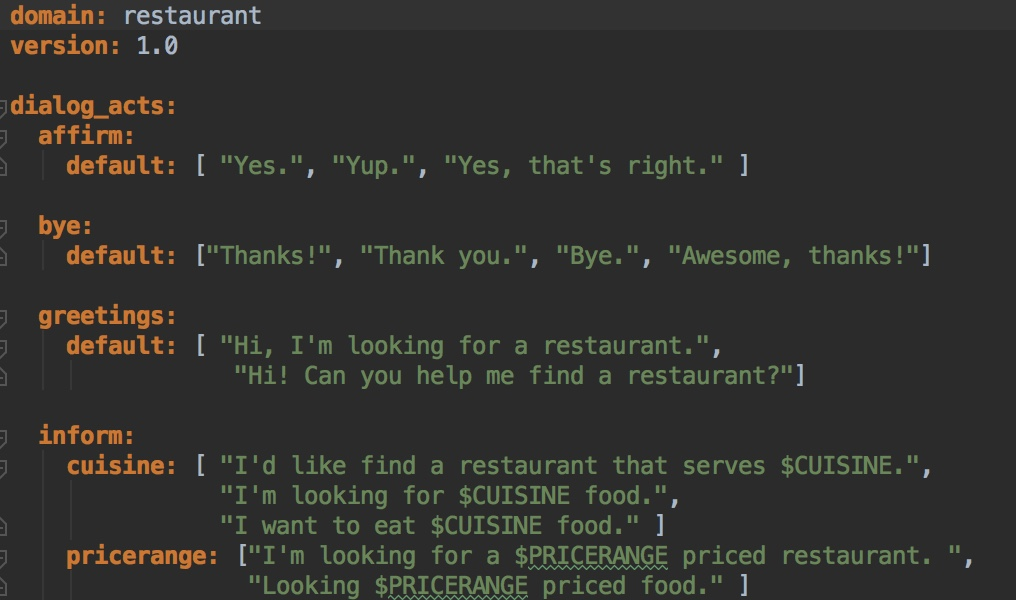
\includegraphics[scale=.35]{diagrams/nlg_template_restaurant.jpeg}
	\caption{ NLG template for user simulator. }
	\label{fig:res_nlg}
\end{figure}

The \textit{get utterance} method in the user simulator will be passed a dialog action object which contains the dialog act and a list dialog parameters. We first look up the dialog act in the nlg template dictionary. Next, we look up the slot values (if any) for the specific language templates. The slot values are passed through the dialog params property of the \textit{DialogAction} object. Additionally, language templates that have multiple slot type are indexed by the combination of the slot types into a single string. We take the slot types, lowercase them, arrange them by alphabetical order, and concatenate them together with a comma separator into a single string. For example, \textit{I want \$PRICE \$CUISINE} would be indexed by the string \textit{cuisine,price}. Finally, we randomly sample the list from the list of potential language templates, substitute slot values, and return a generated natural language utterance. 


\subsection{Neural Model for NLG}

We follow the same process for developing the neural-machine translation model for nlg as we did for the nlu model. We swap the input and target. The model takes in a dialog action and returns a natural language utterance. The \cite{brownlee_2017} model achieved a cross-validation accuracy of .45 and had an accuracy of .34 against the test set. The OpenNMT model had an improved cross-validation accuracy of .65 and test accuracy of .56.  

\section{Dialog Agent Implementation}

The restaurant agent was developed to illustrate how to incorporate an external dialog agent into the simulation framework. Since we do not have an existing restaurant recommendation agent, we developed a simple rule-based agent. The goal of the agent is to capture all of the user's preferences and then make a suggestion from its knowledge base of Cambridge restaurants. Like the user simulator, the public facing methods the dialog manager interacts with are \textit{next} and \textit{get utterance}. 

For the restaurant agent, we follow a simple rule-based approach. The agent expects to interact with the following dialog acts: greetings, affirm, negate, request, inform, bye. In situations where the agent encounters an unknown dialog act, it will repeat its last dialog act. At the beginning of conversation round, dialog agent internally resets its own internal goal (\ref{fig:ex_res_agent_goal}). 

 \begin{figure}[h!]
 	\begin{lstlisting}
 	inform_slots: None
 	request_slots:
 		cuisine: UNK
 		area: UNK
 		pricerange: UNK 	
 	\end{lstlisting}
 	\caption{ Example goal for restaurant agent.}
 	\label{fig:ex_res_agent_goal}
 \end{figure}

If the restaurant agent goes first, it issues a greetings action. If the agent is not responding to the user, it will sequentially pop one item from its request slots and issue a request dialog act. Once the restaurant agent has collected information from the user, it will attempt to make a suggestion from the knowledge base stored in the domain object. This is accomplished by calling the \textit{get suggestion} method provided by the domain object.

The dialog agent's dialog action space is limited. The agent will respond with one of the following dialog acts:
\begin{itemize}
	\item greetings: the agent will greet the user and list its services
	\item request: the agent will ask a probing question to elicit the user's preferences
	\item inform: the agent will supply the user with information (usually tied to the user's request slots)
	\item confirm: the agent will ask the user to confirm if it understood the user's intent 
	\item bye: the agent will end the conversation  
\end{itemize}

\section{Simulating Dialogs with Socrates Sim}
Once we have all the component pieces, we are able to run Socrates Sim. To run the simulations, we first create a simulation configuration file (Figure \ref{fig:restaurant_sim_config }). As we mentioned above, the nlg and nlu processes are abstracted from the user simulator. We are able to swap in the different approaches for both nlg and nlu by modifying the \textit{nlg\_class} and \textit{nlu\_class} property of the configuration file. At load time, these classes are dynamically loaded and the user simulator is able to seamlessly use them without explicit integration code. 

\begin{figure}[h!]
	\centering
	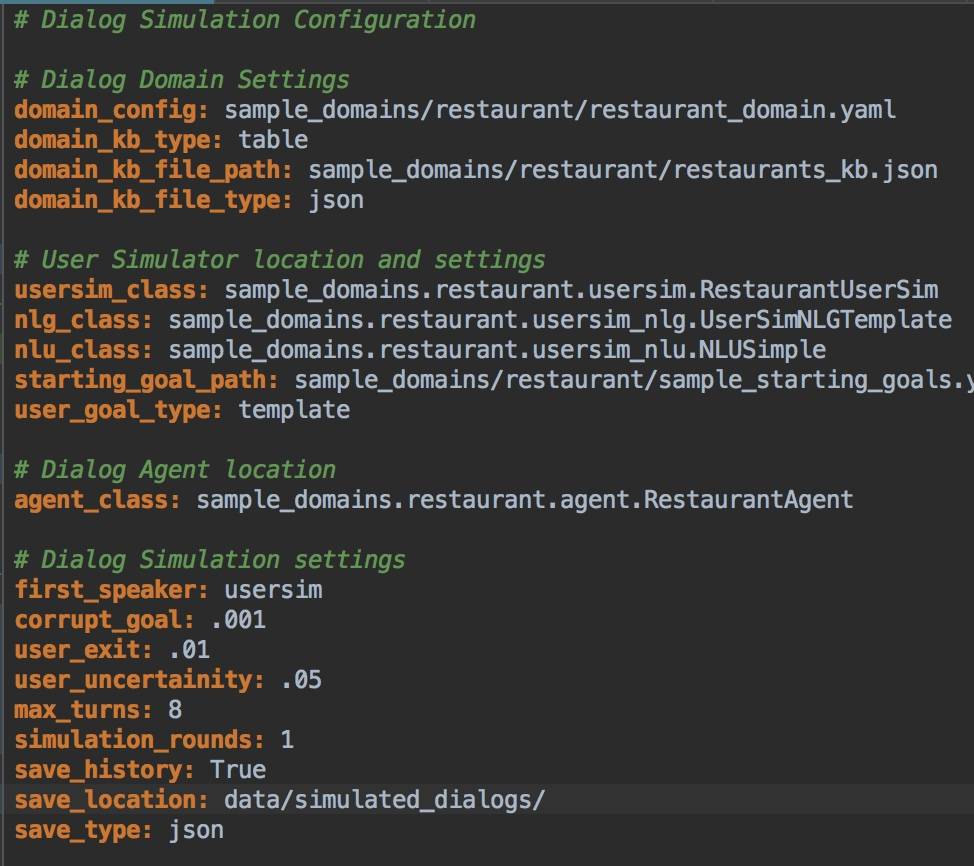
\includegraphics[scale=.35]{diagrams/restaurant_sim_config.jpeg}
	\caption{ Simulation configuration file. }
	\label{fig:restaurant_sim_config }
\end{figure}

The user simulator and dialog agent classes are also dynamically loaded. If the researcher has alternative speaker classes, they can easily plug them in by updating the \textit{usersim\_class} or \textit{agent\_class} properties of the configuration file.

In the Dialog Simulation settings section, we lay out the different simulation settings. For this demonstration, we run a single simulation with various user simulator settings. Additionally, we save the generated dialogs to a json file. Finally, we run the simulation using the command line invocation. Figure \ref{fig:ex_output} shows two examples of dialogs generated by the simulator. 

\begin{figure}[h!]
	\centering
	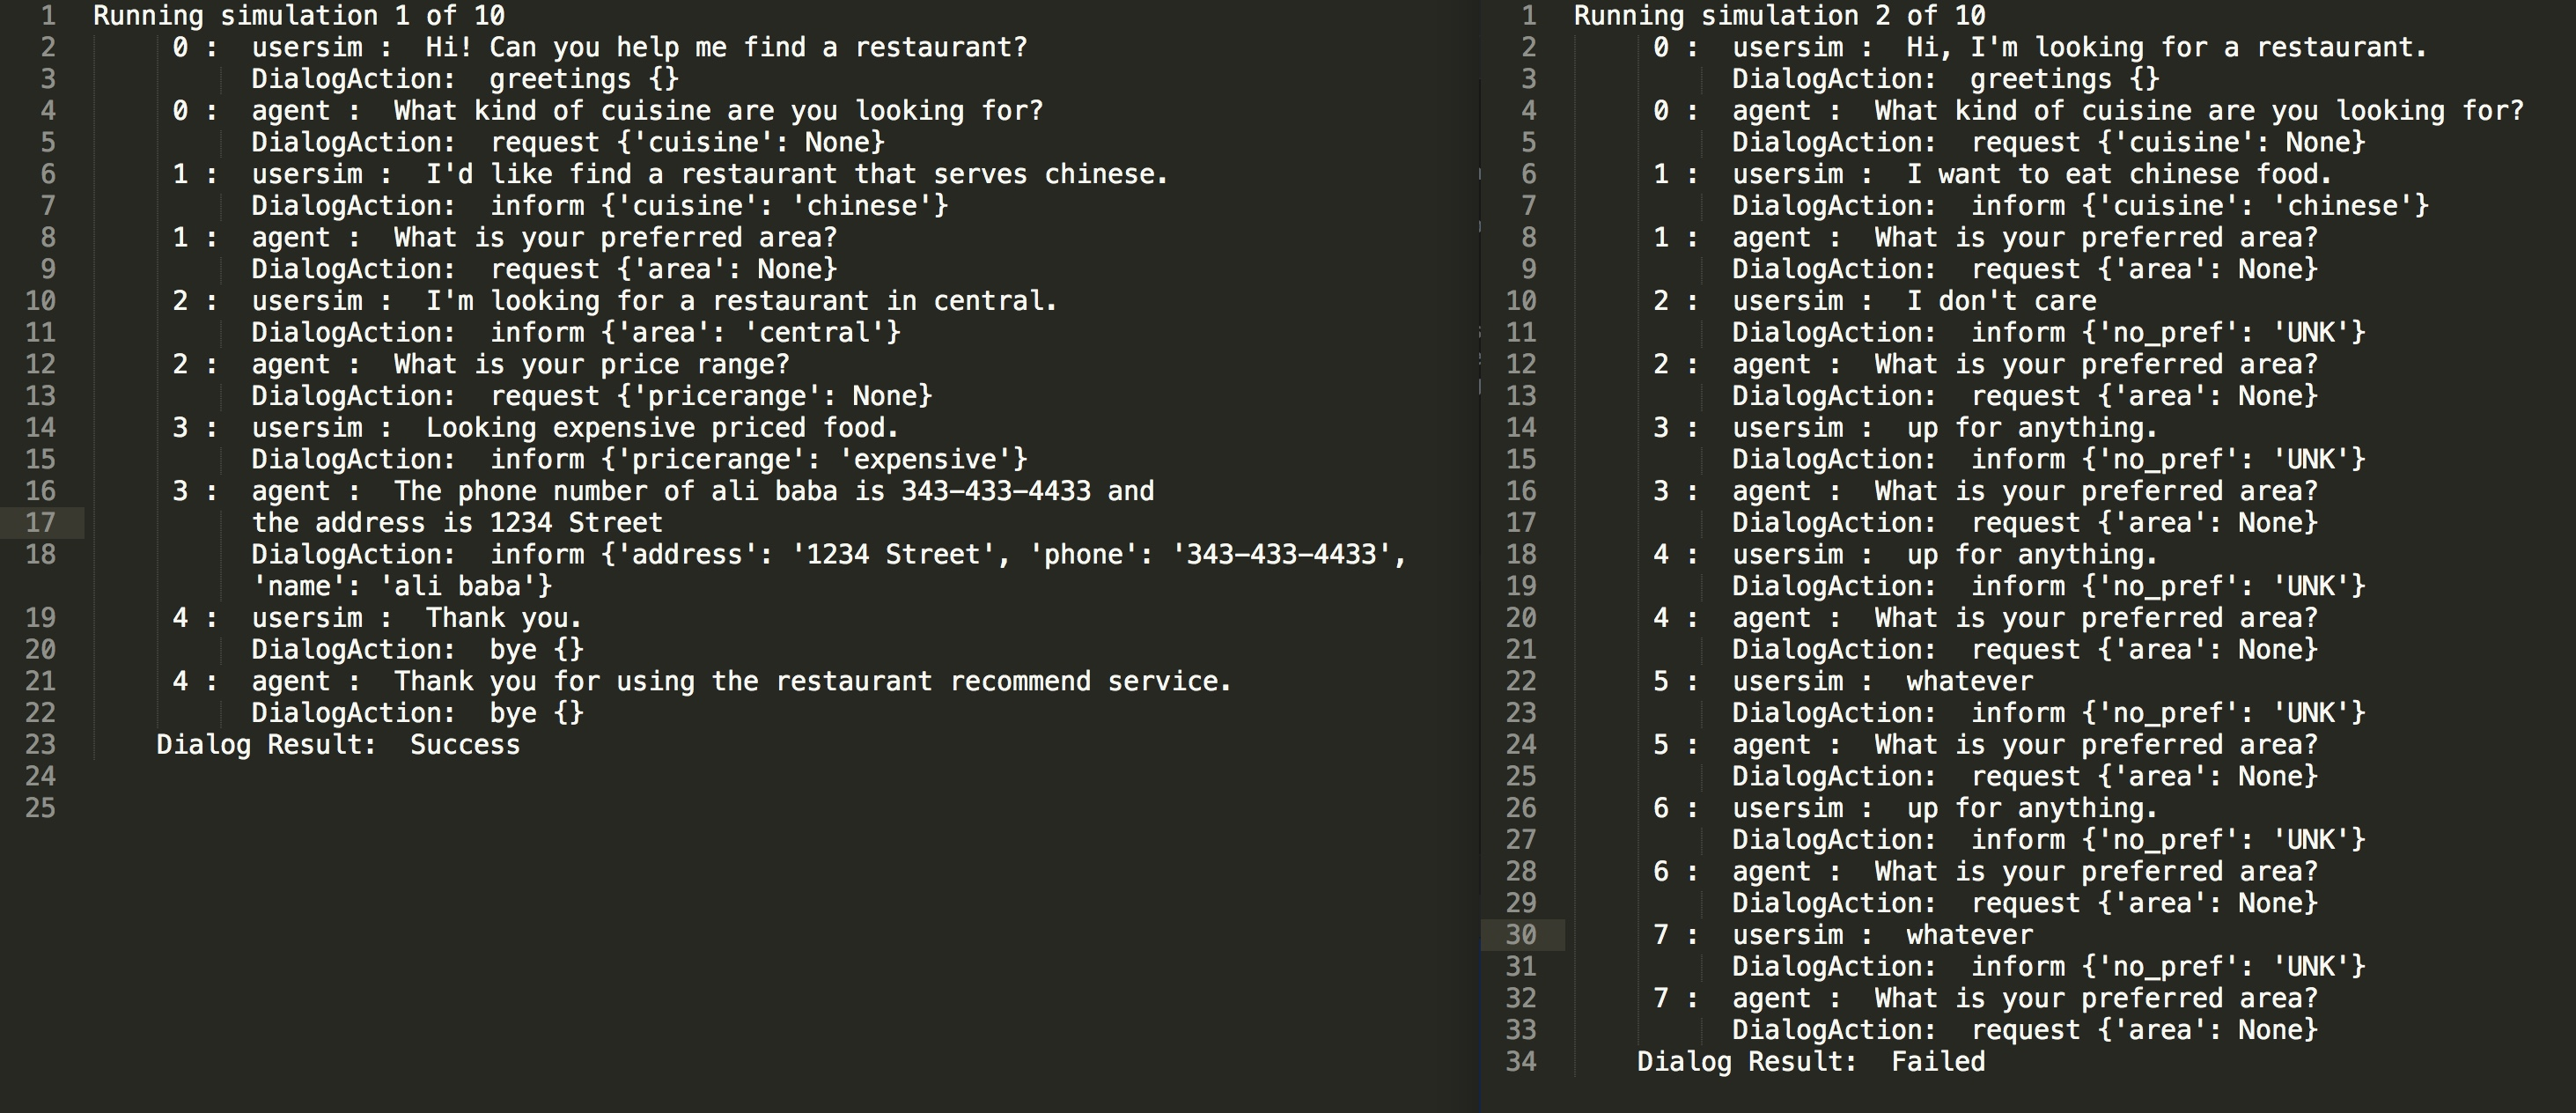
\includegraphics[scale=.16]{diagrams/sample_res_output.jpeg}
	\caption{ Sample dialog generated by Socrates Sim.}
	\label{fig:ex_output}
\end{figure}



%%% Local Variables: 
%%% mode: latex
%%% TeX-master: "main"
%%% End: 
